\section{Integral de línea en campos vectoriales}

La integral de línea respecto de $ds$ acumula valores escalares a lo largo de una curva. Cuando a cada punto se le asigna una fuerza $\mathbf{F}$, interesa además la dirección del recorrido: una fuerza puede favorecer el movimiento, oponerse a él o ser perpendicular a él. La cantidad que registra este efecto es el trabajo.

\subsection{Trabajo de una fuerza a lo largo de una trayectoria}

Para una fuerza constante $\mathbf{F}$ y un desplazamiento rectilíneo $\Delta\vec r$, el trabajo es $\mathbf{F}\cdot\Delta\vec r$. Si $\theta$ es el ángulo entre ambos vectores, se tiene
\[
\mathbf{F}\cdot\Delta\vec r=\|\mathbf{F}\|\,\|\Delta\vec r\|\cos\theta.
\]
Solo contribuye la componente de la fuerza paralela al desplazamiento. El trabajo es positivo si la fuerza favorece el recorrido, negativo si se opone a él y nulo si es perpendicular. Si la fuerza varía con la posición o la trayectoria se curva, esta expresión se aplica a tramos pequeños y luego se suman sus contribuciones.

Sea $C$ una curva espacial orientada desde $P_0$ hasta $P_n$, dividida mediante los puntos $P_0,P_1,\ldots,P_n$. En el tramo $i$ se elige $P_i^*$, y $\Delta\vec r_i=\overrightarrow{P_{i-1}P_i}$ aproxima el desplazamiento sobre el arco. El trabajo aproximado es
\[
W_{\mathcal P}=\sum_{i=1}^n\mathbf{F}(P_i^*)\cdot\Delta\vec r_i.
\]

\begingroup
\shorthandoff{>}
\begin{center}
\begin{tikzpicture}[scale=1.05,every node/.style={font=\small}]
    \draw[->,gray!80!black] (0,0) -- (-1.1,-1.25) node[below left] {$x$};
    \draw[->,gray!80!black] (0,0) -- (5.4,-.55) node[right] {$y$};
    \draw[->,gray!80!black] (0,0) -- (0,3.65) node[above] {$z$};
    \node[below left] at (0,0) {$0$};
    \coordinate (Pzero) at (2.5,-1.45);
    \coordinate (Pprev) at (2.25,2.05);
    \coordinate (Pfinal) at (4.8,.55);
    \coordinate (controlA) at (3.35,2.5);
    \coordinate (controlB) at (4.5,1.55);
    \def\samplepos{.18}
    % Las posiciones se toman directamente de cada tramo de Bézier.
    \draw[blue!75!black,very thick] (Pzero)
        .. controls (1.5,-.75) and (1.1,1.85) .. (Pprev)
        coordinate[pos=.15] (p1) coordinate[pos=.3] (p2)
        coordinate[pos=.45] (p3) coordinate[pos=.6] (p4)
        coordinate[pos=.8] (p5);
    \draw[blue!75!black,very thick] (Pprev)
        .. controls (controlA) and (controlB) .. (Pfinal)
        coordinate[pos=\samplepos] (Psample) coordinate[pos=.4] (Pi)
        coordinate[pos=.65] (p6) coordinate[pos=.85] (p7);
    \foreach \p in {p1,p2,p3,p4,p5,p6,p7}
        \fill[blue!75!black] (\p) circle (1.7pt);
    \fill[blue!75!black] (Pzero) circle (2pt) node[below right] {$P_0$};
    \fill[blue!75!black] (Pfinal) circle (2pt) node[right] {$P_n$};
    \fill[blue!75!black] (Pprev) circle (2pt) node[above left] {$P_{i-1}$};
    \fill[blue!75!black] (Pi) circle (2pt) node[below right] {$P_i$};
    \fill[orange!85!black] (Psample) circle (2.2pt) node[below=5pt] {$P_i^*$};
    \draw[orange!85!black,very thick,->] (Pprev) -- (Pi)
        node[midway,below=14pt] {$\Delta\vec r_i$};
    \draw[->,red!75!black,very thick] (Psample) -- +(-.4,1.05)
        node[above left] {$\mathbf{F}(P_i^*)$};
    % El segmento entre d0 y d1 tiene la dirección de la derivada de Bézier.
    \coordinate (q0) at ($(Pprev)!\samplepos!(controlA)$);
    \coordinate (q1) at ($(controlA)!\samplepos!(controlB)$);
    \coordinate (q2) at ($(controlB)!\samplepos!(Pfinal)$);
    \coordinate (d0) at ($(q0)!\samplepos!(q1)$);
    \coordinate (d1) at ($(q1)!\samplepos!(q2)$);
    \coordinate (tangentDirection) at ($(Psample)+(d1)-(d0)$);
    \draw[->,blue!55!black,thick] (Psample) -- ($(Psample)!1cm!(tangentDirection)$)
        node[above right] {$\mathbf{T}(P_i^*)$};
\end{tikzpicture}
\end{center}
\endgroup

La figura representa un tramo de una curva espacial. La flecha naranja va del punto inicial al final del tramo, al reducir el tramo $\Delta\vec r_i$, su dirección se aproxima a la tangente unitaria $\mathbf{T}(P_i^*)$. La flecha roja es la fuerza del campo vectorial en esa localidad. El producto punto mide la componente de esa fuerza en la dirección de avance, multiplicada por la longitud del desplazamiento.

\begin{mydefinition}{Trabajo e integral de línea de un campo vectorial}
Sea $C$ una curva orientada, regular por partes, contenida en un dominio $D\subseteq\mathbb R^n$, y sea $\mathbf{F}:D\to\mathbb R^n$ continua. El trabajo de $\mathbf{F}$ a lo largo de $C$ se define por
\[
W_C=\int_C\mathbf{F}\cdot d\vec r
=\lim_{\|\mathcal P\|\to0}
\sum_{i=1}^n\mathbf{F}(P_i^*)\cdot\Delta\vec r_i,
\]
donde $\|\mathcal P\|$ es la longitud del arco más largo de la partición. La orientación determina el orden de los puntos de cada tramo.
\end{mydefinition}

En cada tramo regular, $d\vec r=\mathbf{T}\,ds$ y, por tanto,
\[
dW=\mathbf{F}\cdot d\vec r
=\mathbf{F}\cdot\mathbf{T}\,ds
=\|\mathbf{F}\|\cos\theta\,ds.
\]
Aquí $\theta$ es el ángulo entre $\mathbf{F}$ y la tangente orientada. A diferencia de $\int_C f\,ds$, cambiar el sentido de recorrido cambia el signo de $\int_C\mathbf{F}\cdot d\vec r$.

\subsection{Forma diferencial y cálculo mediante una parametrización}

Si $\vec r(t)=(x(t),y(t),z(t))$, $a\leq t\leq b$, recorre $C$ en el sentido indicado, entonces $d\vec r=\vec r\,'(t)\,dt$. La suma anterior se convierte en una integral de una variable:
\begin{mytheorem}{Cálculo de la integral de línea vectorial}
Si $\vec r:[a,b]\to D$ es regular por partes y $\mathbf{F}$ es continua sobre $C$, entonces
\[
\int_C\mathbf{F}\cdot d\vec r
=\int_a^b\mathbf{F}(\vec r(t))\cdot\vec r\,'(t)\,dt.
\]
Si $C$ consta de varios tramos orientados, se suman las integrales de cada tramo.
\end{mytheorem}

En un tramo regular, $d\vec r=\vec r\,'(t)\,dt$ y $ds=\|\vec r\,'(t)\|\,dt$; así, $\mathbf{T}=\vec r\,'/\|\vec r\,'\|$ proporciona también la fórmula anterior a partir de $\mathbf{F}\cdot\mathbf{T}\,ds$. Para $\mathbf{F}=\langle P,Q\rangle$ en el plano o $\mathbf{F}=\langle P,Q,R\rangle$ en el espacio se obtiene la forma diferencial
\[
\int_C\mathbf{F}\cdot d\vec r
=\int_C P\,dx+Q\,dy
\qquad\text{o}\qquad
\int_C\mathbf{F}\cdot d\vec r
=\int_C P\,dx+Q\,dy+R\,dz,
\]
respectivamente. En esta escritura $dx=x'(t)\,dt$, $dy=y'(t)\,dt$ y $dz=z'(t)\,dt$ no son elementos de longitud positivos como en la integral de linea de una función escalar. Si $-C$ denota el mismo camino recorrido en sentido inverso, un cambio de variable decreciente da
\[
\int_{-C}\mathbf{F}\cdot d\vec r=-\int_C\mathbf{F}\cdot d\vec r.
\]

En las figuras siguientes, la curva es azul y las flechas magenta indican el campo.

\begin{samepage}
\paragraph{Ejemplo 1. Un segmento en el plano}
Sea $\mathbf{F}(x,y)=\langle y,x\rangle$ y sea $C$ el segmento de $(0,0)$ a $(1,2)$. Se usa $\vec r(t)=(t,2t)$, $0\leq t\leq1$.
\begingroup
\shorthandoff{>}
\begin{center}
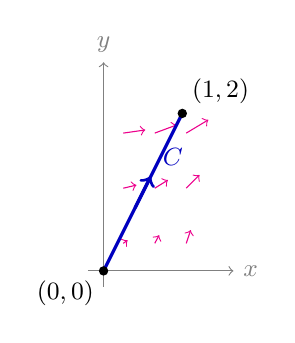
\begin{tikzpicture}[scale=1.0,every node/.style={font=\small}]
    \draw[->,gray] (-.2,0) -- (1.65,0) node[right] {$x$};
    \draw[->,gray] (0,-.2) -- (0,2.65) node[above] {$y$};
    \foreach \xx in {.25,.65,1.05} {
        \foreach \yy in {.35,1.05,1.75} {
            \draw[->,magenta,thin] (\xx,\yy)
                -- ++({.16*\yy},{.16*\xx});
        }
    }
    \draw[blue!75!black,very thick] (0,0) -- (1,2);
    \draw[->,blue!75!black,very thick] (.4,.8) -- (.6,1.2);
    \fill (0,0) circle (1.7pt) node[below left] {$(0,0)$};
    \fill (1,2) circle (1.7pt) node[above right] {$(1,2)$};
    \node[blue!75!black,right] at (.63,1.45) {$C$};
\end{tikzpicture}
\end{center}
\endgroup
\end{samepage}

Al aumentar $t$, se avanza del origen hacia $(1,2)$. Además,
\[
\mathbf{F}(\vec r(t))=\langle2t,t\rangle,
\qquad \vec r\,'(t)=\langle1,2\rangle.
\]
Por tanto, $\int_C\mathbf{F}\cdot d\vec r=\int_0^1(2t+2t)\,dt=2$. La fuerza y el desplazamiento cambian a lo largo del segmento, aunque la dirección de este sea constante.

\begin{samepage}
\paragraph{Ejemplo 2. Una parábola en el plano}
Sea $\mathbf{F}(x,y)=\langle-y,x\rangle$ y recórrase $y=x^2$ desde $(0,0)$ hasta $(1,1)$. Se usa la parametrización $\vec r(t)=(t,t^2)$, $0\leq t\leq1$.
\begingroup
\shorthandoff{>}
\begin{center}
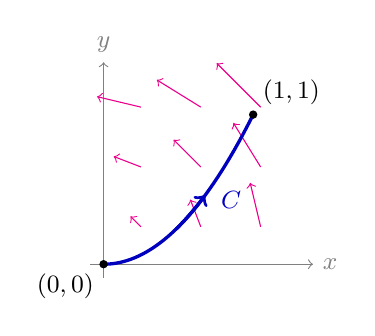
\begin{tikzpicture}[scale=1.9,every node/.style={font=\small}]
    \draw[->,gray] (-.09,0) -- (1.4,0) node[right] {$x$};
    \draw[->,gray] (0,-.09) -- (0,1.35) node[above] {$y$};
    \foreach \xx in {.25,.65,1.05} {
        \foreach \yy in {.25,.65,1.05} {
            \draw[->,magenta,thin] (\xx,\yy)
                -- ++({-.28*\yy},{.28*\xx});
        }
    }
    \draw[blue!75!black,very thick,domain=0:1,samples=60] plot (\x,{\x*\x});
    \draw[->,blue!75!black,very thick,domain=.48:.68,samples=20] plot (\x,{\x*\x});
    \fill (0,0) circle (.8pt) node[below left] {$(0,0)$};
    \fill (1,1) circle (.8pt) node[above right] {$(1,1)$};
    \node[blue!75!black,right] at (.72,.43) {$C$};
\end{tikzpicture}
\end{center}
\endgroup
\end{samepage}

El arco se recorre hacia valores crecientes de $x$. Para calcular el trabajo,
\begin{align*}
\int_C\mathbf{F}\cdot d\vec r
&=\int_0^1\langle-t^2,t\rangle\cdot\langle1,2t\rangle\,dt\\
&=\int_0^1t^2\,dt=\frac13.
\end{align*}
\begin{samepage}
\paragraph{Ejemplo 3. Una hélice en el espacio}
Sea $\mathbf{F}(x,y,z)=\langle-y,x,z\rangle$ y sea $C$ una vuelta de la hélice $\vec r(t)=(\cos t,\sin t,t)$, $0\leq t\leq2\pi$.
\begingroup
\shorthandoff{>}
\begin{center}
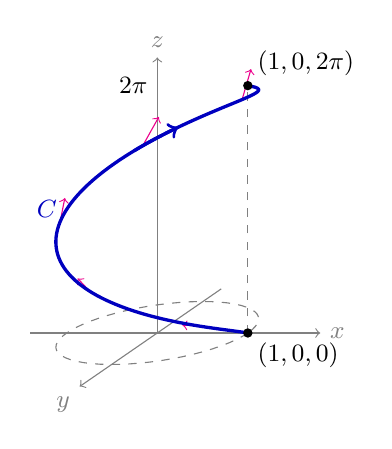
\begin{tikzpicture}[x={(1.15cm,0cm)},y={(-.58cm,-.4cm)},z={(0cm,.5cm)},every node/.style={font=\small}]
    \draw[gray,dashed,domain=0:360,samples=60] plot ({cos(\x)},{sin(\x)},0);
    \draw[gray,dashed] (1,0,0) -- (1,0,{2*pi});
    \draw[->,gray] (-1.4,0,0) -- (1.8,0,0) node[right] {$x$};
    \draw[->,gray] (0,-1.4,0) -- (0,1.7,0) node[below left] {$y$};
    \draw[->,gray] (0,0,0) -- (0,0,7) node[above] {$z$};
    \foreach \ang in {40,105,170,235,300} {
        \draw[->,magenta,thin]
            ({cos(\ang)},{sin(\ang)},{\ang*pi/180})
            -- ++({-.16*sin(\ang)},{.16*cos(\ang)},{.16*\ang*pi/180});
    }
    \draw[blue!75!black,very thick,domain=0:360,samples=120]
        plot ({cos(\x)},{sin(\x)},{\x*pi/180});
    \draw[->,blue!75!black,very thick,domain=230:255,samples=12]
        plot ({cos(\x)},{sin(\x)},{\x*pi/180});
    \fill (1,0,0) circle (1.7pt) node[below right] {$(1,0,0)$};
    \fill (1,0,{2*pi}) circle (1.7pt) node[above right] {$(1,0,2\pi)$};
    \node[left] at (0,0,{2*pi}) {$2\pi$};
    \node[blue!75!black,left] at (-1,0,{pi}) {$C$};
\end{tikzpicture}
\end{center}
\endgroup

La proyección de $C$ sobre el plano $xy$ es la circunferencia unitaria y la altura aumenta de $0$ a $2\pi$.\par
\end{samepage}
En el cálculo se obtiene
\begin{align*}
\mathbf{F}(\vec r(t))\cdot\vec r\,'(t)
&=\langle-\sin t,\cos t,t\rangle
\cdot\langle-\sin t,\cos t,1\rangle\\
&=\sin^2t+\cos^2t+t=1+t,
\end{align*}
de donde $\int_C\mathbf{F}\cdot d\vec r=\int_0^{2\pi}(1+t)\,dt=2\pi+2\pi^2$. La componente vertical de la fuerza también realiza trabajo porque la hélice asciende.

\subsection{Integrales de línea sobre trayectorias cerradas}

Una trayectoria es cerrada si sus puntos inicial y final coinciden: $\vec r(a)=\vec r(b)$. Puede tener esquinas si es regular por partes. La integral se escribe
\[
\oint_C\mathbf{F}\cdot d\vec r
=\int_a^b\mathbf{F}(\vec r(t))\cdot\vec r\,'(t)\,dt.
\]
\begin{samepage}
En el plano, el sentido antihorario se llama orientación positiva. Una integral cerrada mide el trabajo neto tras una vuelta completa; volver al punto inicial no implica que el trabajo sea cero.\par
\end{samepage}

\begin{samepage}
\paragraph{Ejemplo 4. Circulación alrededor de una circunferencia}
Para $\mathbf{F}(x,y)=\langle-y,x\rangle$ y la circunferencia unitaria $C$ orientada en sentido antihorario, se usa $\vec r(t)=(\cos t,\sin t)$, $0\leq t\leq2\pi$.

\begingroup
\shorthandoff{>}
\begin{center}
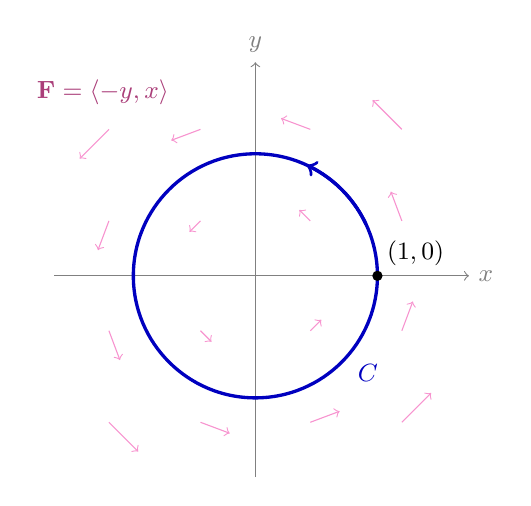
\begin{tikzpicture}[scale=1.55,every node/.style={font=\small}]
    \draw[->,gray] (-1.65,0) -- (1.75,0) node[right] {$x$};
    \draw[->,gray] (0,-1.65) -- (0,1.75) node[above] {$y$};
    % En cada punto, la flecha tiene la dirección de <-y,x>.
    \foreach \xx in {-1.2,-.45,.45,1.2} {
        \foreach \yy in {-1.2,-.45,.45,1.2} {
            \draw[->,magenta!42!white,thin] (\xx,\yy)
                -- ++({-.2*\yy},{.2*\xx});
        }
    }
    \draw[blue!75!black,very thick] (0,0) circle (1);
    \draw[->,blue!75!black,very thick,domain=25:65,samples=20]
        plot ({cos(\x)},{sin(\x)});
    \fill (1,0) circle (1.2pt) node[above right] {$(1,0)$};
    \node[blue!75!black,below right] at (.76,-.65) {$C$};
    \node[magenta!65!black] at (-1.25,1.5) {$\mathbf{F}=\langle-y,x\rangle$};
\end{tikzpicture}
\end{center}
\endgroup

Las flechas del campo son tangentes a las circunferencias centradas en el origen y apuntan en sentido antihorario. Así,
\end{samepage}
\[
\oint_C\mathbf{F}\cdot d\vec r
=\int_0^{2\pi}\langle-\sin t,\cos t\rangle
\cdot\langle-\sin t,\cos t\rangle\,dt
=\int_0^{2\pi}1\,dt=2\pi.
\]
El campo es tangente a la circunferencia y apunta en el sentido de recorrido. Si se invierte la orientación, la integral vale $-2\pi$.

\subsection{Teorema fundamental e independencia de la trayectoria}

Se recuerda que un campo $\mathbf{F}$ es conservativo en un dominio $D$ si existe una función potencial $\varphi$ tal que $\mathbf{F}=\nabla\varphi$ en todo $D$. La función potencial debe estar definida en el dominio por el que pasa la trayectoria.

\begin{mytheorem}{Teorema fundamental de las integrales de línea}
Sea $D\subseteq\mathbb R^n$ un dominio abierto, sea $\varphi:D\to\mathbb R$ de clase $C^1$, y sea $C$ una curva orientada y regular por partes, contenida en $D$, que va de $A$ a $B$. Si $\mathbf{F}=\nabla\varphi$ en $D$, entonces
\[
\int_C\mathbf{F}\cdot d\vec r=\varphi(B)-\varphi(A).
\]
En particular, si $C$ es cerrada, $\displaystyle\oint_C\mathbf{F}\cdot d\vec r=0$.
\end{mytheorem}

\begin{proof}
En cada tramo regular $\vec r:[a,b]\to D$, la regla de la cadena da
\[
\frac{d}{dt}\varphi(\vec r(t))
=\nabla\varphi(\vec r(t))\cdot\vec r\,'(t)
=\mathbf{F}(\vec r(t))\cdot\vec r\,'(t).
\]
Al sustituir esta identidad en la integral de línea parametrizada y aplicar el teorema fundamental del Cálculo de una variable, se obtiene
\begin{align*}
\int_C\mathbf{F}\cdot d\vec r
&=\int_a^b\mathbf{F}(\vec r(t))\cdot\vec r\,'(t)\,dt\\
&=\int_a^b\frac{d}{dt}\varphi(\vec r(t))\,dt\\
&=\left[\varphi(\vec r(t))\right]_a^b\\
&=\varphi(\vec r(b))-\varphi(\vec r(a))\\
&=\varphi(B)-\varphi(A),
\end{align*}
porque $A=\vec r(a)$ y $B=\vec r(b)$. Si $C$ es regular por partes, se aplica este cálculo a cada tramo; al sumar, los valores de $\varphi$ en los extremos interiores se cancelan. Finalmente, cuando $C$ es cerrada se tiene $A=B$, por lo que la diferencia es cero.
\end{proof}

\begin{samepage}
\paragraph{Ejemplo 5. Aplicación del teorema fundamental}
Sea $\mathbf{F}(x,y)=\langle2x,2y+1\rangle$ y sea $C$ el cuarto de la circunferencia unitaria que va de $A=(1,0)$ a $B=(0,1)$ en sentido antihorario. Una parametrización es $\vec r(t)=(\cos t,\sin t)$, $0\leq t\leq\pi/2$.

\begingroup
\shorthandoff{>}
\begin{center}
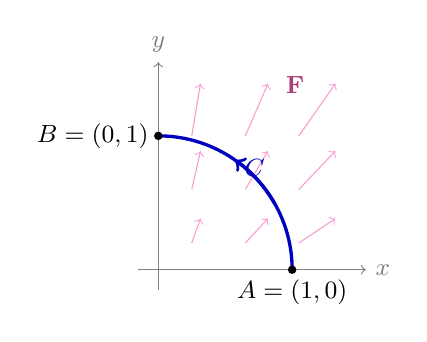
\begin{tikzpicture}[scale=1.7,every node/.style={font=\small}]
    \draw[->,gray] (-.15,0) -- (1.55,0) node[right] {$x$};
    \draw[->,gray] (0,-.15) -- (0,1.55) node[above] {$y$};
    \foreach \xx in {.25,.65,1.05} {
        \foreach \yy in {.2,.6,1} {
            \draw[->,magenta!38!white,thin] (\xx,\yy)
                -- ++({.13*2*\xx},{.13*(2*\yy+1)});
        }
    }
    \draw[blue!75!black,very thick] (1,0) arc (0:90:1);
    \draw[->,blue!75!black,very thick] (30:1) arc (30:55:1);
    \fill (1,0) circle (.9pt) node[below] {$A=(1,0)$};
    \fill (0,1) circle (.9pt) node[left] {$B=(0,1)$};
    \node[blue!75!black] at (.72,.76) {$C$};
    \node[magenta!65!black,right] at (.88,1.38) {$\mathbf{F}$};
\end{tikzpicture}
\end{center}
\endgroup
\end{samepage}

Como
\[
\varphi(x,y)=x^2+y^2+y
\qquad\text{satisface}\qquad
\nabla\varphi=\mathbf{F},
\]
no es necesario evaluar la integral parametrizada. El teorema fundamental da directamente
\[
\int_C\mathbf{F}\cdot d\vec r
=\varphi(0,1)-\varphi(1,0)
=2-1=1.
\]
La figura muestra que la fuerza no es tangente a $C$ en todos sus puntos; aun así, el trabajo total se determina únicamente mediante el potencial en los extremos.

\begin{mytheorem}{Campos conservativos e independencia de la trayectoria}
Sea $D\subseteq\mathbb R^2$ una región abierta y conexa, y sea $\mathbf{F}=\langle M,N\rangle:D\to\mathbb R^2$ continua. El campo $\mathbf{F}$ es conservativo en $D$ si y solo si su integral de línea es independiente de la trayectoria. Es decir, para cualesquiera puntos $A,B\in D$ y cualesquiera curvas regulares por partes $C_1,C_2\subseteq D$ orientadas desde $A$ hasta $B$, se cumple
\[
\int_{C_1}\mathbf{F}\cdot d\vec r
=\int_{C_2}\mathbf{F}\cdot d\vec r.
\]
\end{mytheorem}

\begin{proof}
Supóngase primero que $\mathbf{F}$ es conservativo, de modo que existe $\varphi$ con $\mathbf{F}=\nabla\varphi$ en $D$. El teorema fundamental se aplica a cada curva y da
\[
\int_{C_1}\mathbf{F}\cdot d\vec r
=\varphi(B)-\varphi(A)
=\int_{C_2}\mathbf{F}\cdot d\vec r.
\]
Por tanto, la integral solo depende de los extremos.

Para demostrar el recíproco, supóngase que la integral es independiente de la trayectoria. Se fija un punto $A_0=(x_0,y_0)\in D$ y, para cada $X=(x,y)\in D$, se define
\[
\varphi(X)=\int_{C_X}\mathbf{F}\cdot d\vec r,
\]
donde $C_X$ es cualquier curva regular por partes contenida en $D$ que vaya de $A_0$ a $X$. Como $D$ es abierto y conexo, tales curvas existen; además, la independencia de la trayectoria garantiza que $\varphi(X)$ no depende de la curva elegida.

Como $D$ es abierto, para $h$ suficientemente pequeño el segmento horizontal desde $(x,y)$ hasta $(x+h,y)$ está contenido en $D$. Puede calcularse $\varphi(x+h,y)$ siguiendo primero una curva desde $A_0$ hasta $(x,y)$ y después este segmento. La independencia de la trayectoria permite escribir
\begin{align*}
\varphi(x+h,y)-\varphi(x,y)
&=\int_x^{x+h}M(s,y)\,ds.
\end{align*}
Al dividir entre $h$ y tomar el límite, la continuidad de $M$ da
\[
\varphi_x(x,y)
=\lim_{h\to0}\frac{1}{h}\int_x^{x+h}M(s,y)\,ds
=M(x,y).
\]

De manera análoga, para un segmento vertical desde $(x,y)$ hasta $(x,y+k)$ se tiene
\[
\varphi(x,y+k)-\varphi(x,y)
=\int_y^{y+k}N(x,s)\,ds,
\]
y, en consecuencia,
\[
\varphi_y(x,y)
=\lim_{k\to0}\frac{1}{k}\int_y^{y+k}N(x,s)\,ds
=N(x,y).
\]
Por lo tanto,
\[
\nabla\varphi(x,y)
=\langle\varphi_x(x,y),\varphi_y(x,y)\rangle
=\langle M(x,y),N(x,y)\rangle
=\mathbf{F}(x,y),
\]
de modo que $\mathbf{F}$ es conservativo en $D$. El mismo argumento se extiende a $\mathbb R^3$ añadiendo segmentos paralelos al eje $z$.
\end{proof}

La condición de ser conservativo no puede reemplazarse simplemente por que los extremos coincidan. Para reconocer un potencial en el plano, si $\mathbf{F}=\langle P,Q\rangle$, se buscan $\varphi_x=P$ y $\varphi_y=Q$, y en el espacio se añade $\varphi_z=R$. Si $P$ y $Q$ tienen derivadas parciales continuas, la igualdad $P_y=Q_x$ es necesaria para que exista un potencial de clase $C^2$, pero en un dominio con agujeros no basta por sí sola. Una vez encontrado $\varphi$, se verifica $\nabla\varphi=\mathbf{F}$ en todo el dominio pertinente.

\begin{samepage}
\paragraph{Ejemplo 6. Potencial conocido y dos trayectorias}
Sea $\varphi(x,y)=x^2y+\sin x+y^2$ y $\mathbf{F}=\nabla\varphi=\langle2xy+\cos x,x^2+2y\rangle$. La trayectoria $C_1$ va de $A=(0,0)$ a $B=(1,1)$ primero por un segmento horizontal y luego por uno vertical; $C_2$ es la diagonal entre los mismos puntos.

\begingroup
\shorthandoff{>}
\begin{center}
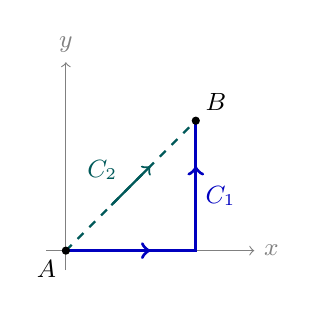
\begin{tikzpicture}[scale=1.65,every node/.style={font=\small}]
    \draw[->,gray] (-.15,0) -- (1.45,0) node[right] {$x$};
    \draw[->,gray] (0,-.15) -- (0,1.45) node[above] {$y$};
    \draw[blue!75!black,very thick] (0,0) -- (1,0) -- (1,1);
    \draw[->,blue!75!black,very thick] (.35,0) -- (.65,0);
    \draw[->,blue!75!black,very thick] (1,.35) -- (1,.65);
    \draw[teal!70!black,thick,dashed] (0,0) -- (1,1);
    \draw[->,teal!70!black,thick] (.35,.35) -- (.65,.65);
    \fill (0,0) circle (.9pt) node[below left] {$A$};
    \fill (1,1) circle (.9pt) node[above right] {$B$};
    \node[blue!75!black,right] at (1,.42) {$C_1$};
    \node[teal!70!black,above left] at (.47,.47) {$C_2$};
\end{tikzpicture}
\end{center}
\endgroup
\end{samepage}

Al estar definida $\varphi$ en todo $\mathbb R^2$, el teorema fundamental da para ambas trayectorias
\[
\int_{C_1}\mathbf{F}\cdot d\vec r
=\varphi(1,1)-\varphi(0,0)
=2+\sin1
=\int_{C_2}\mathbf{F}\cdot d\vec r.
\]

\begin{samepage}
\paragraph{Ejemplo 7. Construcción de un potencial en el plano}
Considérese $\mathbf{F}(x,y)=\langle2xy+1,x^2+2y\rangle$. De $\varphi_x=2xy+1$ se obtiene $\varphi=x^2y+x+g(y)$. La condición $\varphi_y=x^2+2y$ exige $g'(y)=2y$, de modo que puede tomarse $\varphi=x^2y+x+y^2$. La figura muestra dos posibles trayectorias desde $A=(0,0)$ hasta $B=(2,1)$.

\begingroup
\shorthandoff{>}
\begin{center}
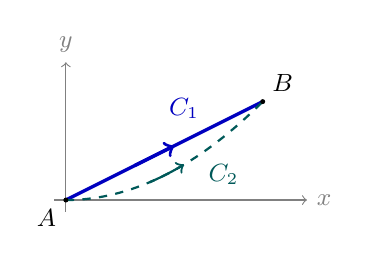
\begin{tikzpicture}[x=1.25cm,y=1.25cm,every node/.style={font=\small}]
    \draw[->,gray] (-.12,0) -- (2.45,0) node[right] {$x$};
    \draw[->,gray] (0,-.12) -- (0,1.4) node[above] {$y$};
    \draw[blue!75!black,very thick] (0,0) -- (2,1);
    \draw[->,blue!75!black,very thick] (.7,.35) -- (1.1,.55);
    \draw[teal!70!black,thick,dashed,domain=0:2,samples=60]
        plot (\x,{\x*\x/4});
    \draw[->,teal!70!black,thick,domain=.85:1.2,samples=15]
        plot (\x,{\x*\x/4});
    \fill (0,0) circle (.9pt) node[below left] {$A$};
    \fill (2,1) circle (.9pt) node[above right] {$B$};
    \node[blue!75!black,above left] at (1.45,.73) {$C_1$};
    \node[teal!70!black,below right] at (1.35,.46) {$C_2$};
\end{tikzpicture}
\end{center}
\endgroup
\end{samepage}

Como el valor depende únicamente de los extremos, para $C=C_1$, $C=C_2$ o cualquier otra trayectoria regular por partes en $\mathbb R^2$ se obtiene
\[
\int_C\mathbf{F}\cdot d\vec r
=\varphi(2,1)-\varphi(0,0)=4+2+1=7.
\]

\begin{samepage}
\paragraph{Ejemplo 8. Independencia de la trayectoria en el espacio}
Sea $\mathbf{F}(x,y,z)=\langle yz+2x,xz,xy+2z\rangle$. La función $\varphi(x,y,z)=xyz+x^2+z^2$ satisface $\nabla\varphi=\mathbf{F}$ en $\mathbb R^3$. En la figura, $C_1$ es el segmento de $A=(0,0,0)$ a $B=(1,2,3)$ y $C_2$ es una trayectoria quebrada con los mismos extremos.

\begingroup
\shorthandoff{>}
\begin{center}
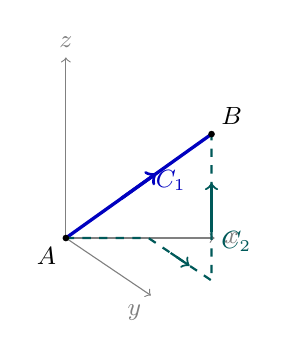
\begin{tikzpicture}[x={(1.05cm,0cm)},y={(.4cm,-.27cm)},z={(0cm,.62cm)},every node/.style={font=\small}]
    \draw[->,gray] (0,0,0) -- (1.8,0,0) node[right] {$x$};
    \draw[->,gray] (0,0,0) -- (0,2.7,0) node[below left] {$y$};
    \draw[->,gray] (0,0,0) -- (0,0,3.7) node[above] {$z$};
    \draw[blue!75!black,very thick] (0,0,0) -- (1,2,3);
    \draw[->,blue!75!black,very thick] (.38,.76,1.14) -- (.62,1.24,1.86);
    \draw[teal!70!black,thick,dashed] (0,0,0) -- (1,0,0) -- (1,2,0) -- (1,2,3);
    \draw[->,teal!70!black,thick] (1,.7,0) -- (1,1.3,0);
    \draw[->,teal!70!black,thick] (1,2,1) -- (1,2,2);
    \fill (0,0,0) circle (1.2pt) node[below left] {$A$};
    \fill (1,2,3) circle (1.2pt) node[above right] {$B$};
    \node[blue!75!black,right] at (.55,1.1,1.65) {$C_1$};
    \node[teal!70!black,right] at (1,2,.8) {$C_2$};
\end{tikzpicture}
\end{center}
\endgroup
\end{samepage}

Para cualquiera de las dos trayectorias, y en realidad para cualquier curva regular por partes entre esos extremos,
\[
\int_C\mathbf{F}\cdot d\vec r
=\varphi(1,2,3)-\varphi(0,0,0)=6+1+9=16.
\]

\begin{samepage}
\paragraph{Ejemplo 9. Dos trayectorias con trabajos distintos}
Sea $\mathbf{F}(x,y)=\langle y,0\rangle$ y sean $A=(0,0)$ y $B=(1,1)$. La trayectoria $C_1$ es la diagonal, mientras que $C_2$ va primero de $A$ a $(1,0)$ y después a $B$.

\begingroup
\shorthandoff{>}
\begin{center}
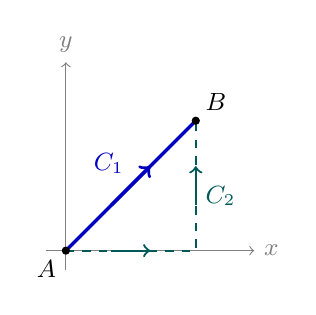
\begin{tikzpicture}[scale=1.65,every node/.style={font=\small}]
    \draw[->,gray] (-.15,0) -- (1.45,0) node[right] {$x$};
    \draw[->,gray] (0,-.15) -- (0,1.45) node[above] {$y$};
    \draw[blue!75!black,very thick] (0,0) -- (1,1);
    \draw[->,blue!75!black,very thick] (.35,.35) -- (.65,.65);
    \draw[teal!70!black,thick,dashed] (0,0) -- (1,0) -- (1,1);
    \draw[->,teal!70!black,thick] (.35,0) -- (.65,0);
    \draw[->,teal!70!black,thick] (1,.35) -- (1,.65);
    \fill (0,0) circle (.9pt) node[below left] {$A$};
    \fill (1,1) circle (.9pt) node[above right] {$B$};
    \node[blue!75!black,above left] at (.52,.52) {$C_1$};
    \node[teal!70!black,right] at (1,.42) {$C_2$};
\end{tikzpicture}
\end{center}
\endgroup
\end{samepage}

En la diagonal, $\vec r(t)=(t,t)$, $0\leq t\leq1$, y se obtiene
\[
\int_{C_1}\mathbf{F}\cdot d\vec r
=\int_0^1\langle t,0\rangle\cdot\langle1,1\rangle\,dt=\frac12.
\]
En $C_2$, se puede probar facilmente que $\int_{C_2}\mathbf{F}\cdot d\vec r=0$. Como los trabajos difieren, $\mathbf{F}$ no es conservativo en $\mathbb R^2$.

\subsection{Conservación de la energía}

En mecánica, si una fuerza conservativa admite una energía potencial $U$ tal que $\mathbf{F}=-\nabla U$, el teorema fundamental expresa su trabajo desde $A$ hasta $B$ como
\[
W_C=U(A)-U(B)=-\Delta U.
\]
El signo negativo indica que la fuerza realiza trabajo positivo cuando disminuye la energía potencial.

Si una partícula de masa constante $m$ satisface $m\vec r\,''(t)=\mathbf{F}(\vec r(t))$ y esta es la única fuerza que realiza trabajo, su energía cinética es $K=\tfrac12m\|\vec r\,'(t)\|^2$. La regla del producto y la ecuación de movimiento dan
\[
\frac{dK}{dt}=m\vec r\,''(t)\cdot\vec r\,'(t)
=\mathbf{F}(\vec r(t))\cdot\vec r\,'(t)
=-\frac{d}{dt}U(\vec r(t)).
\]
Por ello $K+U$ es constante y $K(B)-K(A)=W_C$. Si actúan otras fuerzas que realizan trabajo, se suma su trabajo al balance de energía.

Por ejemplo, cerca de la superficie terrestre, con el eje $z$ vertical, $\mathbf{F}=\langle0,0,-mg\rangle$ y $U(x,y,z)=mgz$. Al descender una altura $h>0$, la gravedad realiza trabajo $mgh$, independientemente de la forma de la trayectoria, y la energía cinética aumenta en $mgh$ si no intervienen otras fuerzas que realicen trabajo.

\subsection{Ejercicios}
\begin{enumerate}
    \item Para $\mathbf{F}=\langle3,4\rangle$, determine el signo y el valor del trabajo en desplazamientos de longitud $2$ dirigidos, respectivamente, según $\langle1,0\rangle$, $\langle-1,0\rangle$ y $\langle4/5,-3/5\rangle$.

    \item Calcule $\int_C\mathbf{F}\cdot d\vec r$ para $\mathbf{F}(x,y)=\langle2x,y\rangle$ y el segmento $C$ de $(0,0)$ a $(1,2)$.

    \item Evalúe $\int_C-y\,dx+x\,dy$ sobre el arco $y=x^2$ desde $(0,0)$ hasta $(2,4)$.

    \item Para $\mathbf{F}(x,y)=\langle x+y,x\rangle$, construya una parametrización por tramos de la trayectoria mostrada y calcule su trabajo.
\begingroup
\shorthandoff{>}
\begin{center}
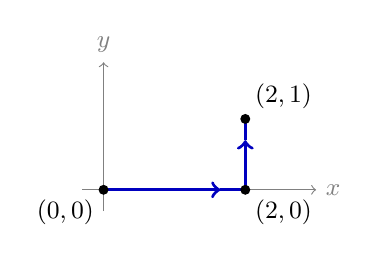
\begin{tikzpicture}[scale=.9,every node/.style={font=\small}]
    \draw[->,gray] (-.3,0)--(3,0) node[right] {$x$};
    \draw[->,gray] (0,-.3)--(0,1.8) node[above] {$y$};
    \draw[blue!75!black,very thick,->] (0,0)--(1.65,0);
    \draw[blue!75!black,very thick] (1.65,0)--(2,0);
    \draw[blue!75!black,very thick,->] (2,0)--(2,.7);
    \draw[blue!75!black,very thick] (2,.7)--(2,1);
    \fill (0,0) circle (2pt) node[below left] {$(0,0)$};
    \fill (2,0) circle (2pt) node[below right] {$(2,0)$};
    \fill (2,1) circle (2pt) node[above right] {$(2,1)$};
\end{tikzpicture}
\end{center}
\endgroup

    \item Calcule el trabajo de $\mathbf{F}(x,y,z)=\langle y,z,x\rangle$ a lo largo del segmento de $(0,0,0)$ a $(1,2,3)$.

    \item Para $\mathbf{F}(x,y)=\langle-y,x\rangle$, construya una parametrización de la trayectoria mostrada y evalúe $\int_C\mathbf{F}\cdot d\vec r$.
\begingroup
\shorthandoff{>}
\begin{center}
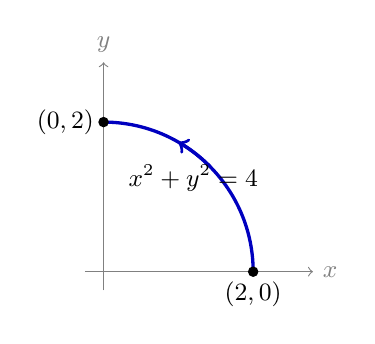
\begin{tikzpicture}[scale=.95,every node/.style={font=\small}]
    \draw[->,gray] (-.25,0)--(2.8,0) node[right] {$x$};
    \draw[->,gray] (0,-.25)--(0,2.8) node[above] {$y$};
    \draw[blue!75!black,very thick] (2,0) arc (0:90:2);
    \draw[blue!75!black,very thick,->] (45:2) arc (45:60:2);
    \fill (2,0) circle (2pt) node[below] {$(2,0)$};
    \fill (0,2) circle (2pt) node[left] {$(0,2)$};
    \node at (1.2,1.25) {$x^2+y^2=4$};
\end{tikzpicture}
\end{center}
\endgroup

    \item Evalúe $\int_C\mathbf{F}\cdot d\vec r$ para $\mathbf{F}(x,y,z)=\langle-y,x,1\rangle$ y $\vec r(t)=(\cos t,\sin t,t)$, $0\leq t\leq\pi$.

    \item Calcule $\oint_C\mathbf{F}\cdot d\vec r$ para $\mathbf{F}(x,y)=\langle-y,x\rangle$ y la circunferencia $x^2+y^2=4$, recorrida una vez en sentido antihorario. Determine después el valor para el sentido contrario.

    \item Para $\mathbf{F}(x,y)=\langle-y,x\rangle$, construya una parametrización por tramos de la trayectoria cerrada mostrada y calcule $\oint_C\mathbf{F}\cdot d\vec r$.
\begingroup
\shorthandoff{>}
\begin{center}
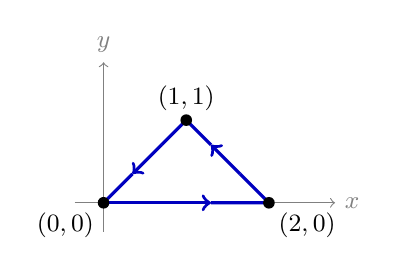
\begin{tikzpicture}[scale=1.05,every node/.style={font=\small}]
    \draw[->,gray] (-.35,0)--(2.8,0) node[right] {$x$};
    \draw[->,gray] (0,-.35)--(0,1.7) node[above] {$y$};
    \draw[blue!75!black,very thick,->] (0,0)--(1.3,0);
    \draw[blue!75!black,very thick] (1.3,0)--(2,0)--(1.65,.35);
    \draw[blue!75!black,very thick,->] (1.65,.35)--(1.3,.7);
    \draw[blue!75!black,very thick] (1.3,.7)--(1,1)--(.7,.7);
    \draw[blue!75!black,very thick,->] (.7,.7)--(.35,.35);
    \draw[blue!75!black,very thick] (.35,.35)--(0,0);
    \fill (0,0) circle (2pt) node[below left] {$(0,0)$};
    \fill (2,0) circle (2pt) node[below right] {$(2,0)$};
    \fill (1,1) circle (2pt) node[above] {$(1,1)$};
\end{tikzpicture}
\end{center}
\endgroup

    \item Demuestre, mediante un cambio de variable, que invertir la orientación de una curva regular por partes cambia el signo de $\int_C\mathbf{F}\cdot d\vec r$.
    \item Sea $\mathbf{F}=\nabla\varphi$ en $\mathbb R^2$, donde $\varphi(x,y)=x^2+y^2$. Evalúe el trabajo desde $(-1,0)$ hasta $(2,3)$ por una trayectoria regular por partes cualquiera.
    \item Encuentre una función potencial para $\mathbf{F}(x,y)=\langle3x^2+2y,2x+2y\rangle$ y calcule el trabajo desde $(0,0)$ hasta $(1,2)$ por cualquier curva regular por partes en $\mathbb R^2$.

    \item Sea $\mathbf{F}=\nabla\varphi$, con $\varphi(x,y)=xy+y^2$. Construya una parametrización por tramos de la trayectoria mostrada, calcule su trabajo directamente y compruébelo mediante el potencial.
\begingroup
\shorthandoff{>}
\begin{center}
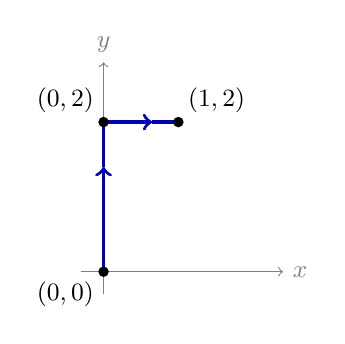
\begin{tikzpicture}[scale=.95,every node/.style={font=\small}]
    \draw[->,gray] (-.3,0)--(2.4,0) node[right] {$x$};
    \draw[->,gray] (0,-.3)--(0,2.8) node[above] {$y$};
    \draw[blue!75!black,very thick,->] (0,0)--(0,1.4);
    \draw[blue!75!black,very thick] (0,1.4)--(0,2);
    \draw[blue!75!black,very thick,->] (0,2)--(.65,2);
    \draw[blue!75!black,very thick] (.65,2)--(1,2);
    \fill (0,0) circle (2pt) node[below left] {$(0,0)$};
    \fill (0,2) circle (2pt) node[above left] {$(0,2)$};
    \fill (1,2) circle (2pt) node[above right] {$(1,2)$};
\end{tikzpicture}
\end{center}
\endgroup

    \item Para $\mathbf{F}(x,y,z)=\langle yz,xz,xy\rangle$, encuentre una función potencial en $\mathbb R^3$ y calcule $\int_C\mathbf{F}\cdot d\vec r$ sobre cualquier trayectoria desde $(1,0,0)$ hasta $(1,2,3)$.

    \item Demuestre que $\oint_C (2x\,dx+2y\,dy)=0$ para toda curva cerrada regular por partes $C$ contenida en $\mathbb R^2$. Indique qué potencial permite aplicar el teorema fundamental.

    \item Para $\mathbf{F}(x,y)=\langle x-y,x\rangle$, compare el trabajo de $(0,0)$ a $(1,1)$ por la diagonal con el trabajo por la trayectoria que va primero a $(1,0)$ y luego a $(1,1)$. Determine si el campo es conservativo en $\mathbb R^2$.

    \item En $D=\mathbb R^2\setminus\{(0,0)\}$, sea
\[
\mathbf{F}(x,y)=\left\langle-\frac{y}{x^2+y^2},\frac{x}{x^2+y^2}\right\rangle.
\]
Evalúe su integral sobre la circunferencia unitaria en sentido antihorario y deduzca si existe un potencial definido en todo $D$.

    \item Una partícula de masa $m$ desciende desde $z=8\,\mathrm m$ hasta $z=3\,\mathrm m$ bajo la fuerza gravitacional constante $\mathbf{F}=\langle0,0,-mg\rangle$. Calcule el trabajo de la gravedad y el cambio de energía potencial, sin fijar la forma de la trayectoria.

    \item Una partícula de masa $m$ se mueve sobre el eje $x$ bajo la fuerza $\mathbf{F}(x,y)=\langle-kx,0\rangle$, donde $k>0$. Encuentre una energía potencial $U$, calcule el trabajo desde $(a,0)$ hasta $(0,0)$ con $a>0$, y determine la rapidez final si parte del reposo y no actúan otras fuerzas que realicen trabajo.

    \item Sea $\varphi:D\subseteq\mathbb R^n\to\mathbb R$ de clase $C^1$ y sea $\mathbf{F}=\nabla\varphi$. Suponga que una curva regular por partes $C$ está contenida en el conjunto de nivel $\varphi(\mathbf{x})=c$.
\begin{enumerate}
    \item Demuestre mediante el teorema fundamental de las integrales de línea que
    \[
    \int_C\mathbf{F}\cdot d\vec r=0.
    \]
    \item Demuestre el mismo resultado directamente: para una parametrización $\vec r(t)$ de cada tramo, derive la identidad $\varphi(\vec r(t))=c$ y relacione el resultado con $\mathbf{F}(\vec r(t))\cdot\vec r\,'(t)$.
    \item Aplique ambas interpretaciones a $\mathbf{F}(x,y,z)=\langle2x,2y,2z\rangle$ y a cualquier curva contenida en la esfera $x^2+y^2+z^2=R^2$. Explique la relación geométrica entre el campo y el vector tangente a la curva.
\end{enumerate}

\end{enumerate}
